\documentclass{article}


\usepackage{authblk}
\usepackage[T1]{fontenc}
\usepackage{indentfirst}
\usepackage{graphicx}
\usepackage{caption}
\usepackage{hyperref}
\usepackage{float}
\usepackage{subcaption}


\begin{document}

\title{Photoluminescence}
\author[1]{Woojin Han}
\affil[1]{Seoul National University, Seoul 151-747, Korea}
\maketitle
\begin{abstract}

\end{abstract}

\section{Introduction}
 In this experiment, photoluminescence(PL) of ruby and rhodamine 590 is measured.
 Analysis between PL peak statics of ruby and temperature is obtained.(\ref{result:temperature_peak_statics})
 The effect by iris of apparatus to PL result is declared, and proved.(\ref{result:iris_effect})
 According to the peak intensity ratio, the mole ratio of $Cr^{3+}$ ion in the ruby is calculated.
 The apparatus data (\cite{ruby_spec}) is also found and compared to the calculation.


\subsection{Photoluminescence:General Theory}
 \label{intro:pl_general_theory}
 Photoluminescence is explained by two different parts, absortion and emission of light.
 Both events occur by the electronic transition through states, embedding the nature of the condensed matter.
 Therefore, the photoluminescence result lead us to measure the band diagram of the crystal.
 Not only the energy level of each band but also lifetime or exact orbital can be measured by the peak statics, such as peak width or intensity ratio.
 \begin{figure}[ht]
    \centering
    \begin{subfigure}[b]{6cm}
        \centering
        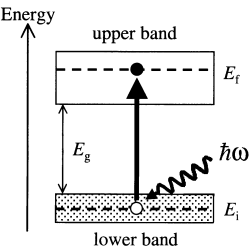
\includegraphics[width=4cm]{../results/intro_energy_absortion.png}
        \caption{}
    \end{subfigure}
    \hfill
    \begin{subfigure}[b]{6cm}
        \centering
        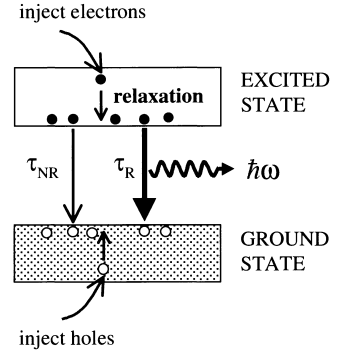
\includegraphics[width=4cm]{../results/intro_energy_emission.png}
        \caption{}
    \end{subfigure}
    \hfill
    \caption{Schematic diagram of (a)light absortion (b)light emission \cite{condensed_matter_optics}}
    \label{fig:pl_intro}
 \end{figure}

 \begin{figure}[ht]
    \centering
    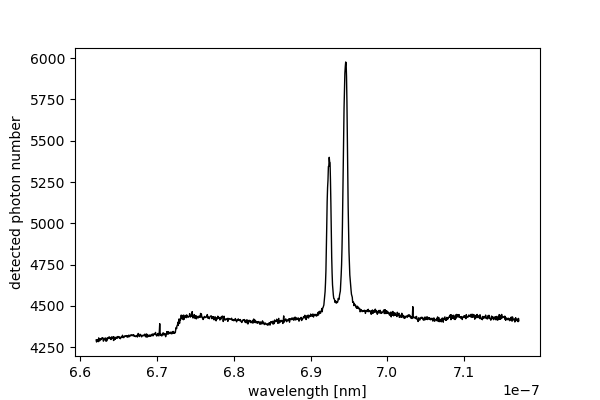
\includegraphics[width=8cm]{../results/Ruby(170.0)_raw_fig.png}
    \caption{photoluminescence results of Ruby in $170.0K$}
    \label{fig:pl_sample}
 \end{figure}
 Fig. \ref{fig:pl_intro}(a) shows the band diagram explaination of light absortion, creating hole in lower band transite to upper band.
 Fig. \ref{fig:pl_intro}(b) is the schematic diagram of light emission, slowly relaxing and emitting light while energy drops between band gap.
 Fig. \ref{fig:pl_sample} is one of the photoluminescence results in this experiment.
 The absorbed light was $532nm$, but we can find out the emitted light have wavelength around $690nm$.
 We can sure the electronic transition is the key mechanisms since the wavelength change can not be explained by scattering, especially for the peak nature.
 Therefore, the peak position is specific to the crystal structure or the molecular shapes.
 But the peak width have two reasons, natural and optical broadening. (\cite{quantum_optics})
 Natural broadening is intrinsic to the transition, caused by lifetime of the states.
 For lifetime $\tau$, the spectral function follows Lorentzian like equation (\ref{equation:natural_broadening}), $\omega$ is the angular frequency of light, and $\Delta \omega$ is full width at half maximum(FWHM) value which is related with lifetime.
 \begin{equation}
   g(\omega) = \frac{\Delta \omega}{2 \pi} \frac{1}{(\omega-\omega_0)^2 + (\Delta \omega/2)^2},\, \Delta \omega = \frac{1}{\tau}
   \label{equation:natural_broadening}
 \end{equation}
 And by the spectral effects by spectroscopy itself, the Gaussian shape optical broadening is inevitable.
 Therefore, I assume that the detected photoluminescence spectroscopy data will follow Voigt profile, which is a convolution results of Lorentzian and Gaussian function.
 \subsection{Ruby}
 \label{intro:ruby}
 

\subsection{Rhodamine 590(R590)}



\section{Methods}

\section{Results and Discussion}
\subsection{photoluminescence result fitting method}
\label{result:iris_effect}

\subsection{Ruby PL result by temperature}
\label{result:temperature_peak_statics}



\section{Summary}

\cite{something}
\bibliography{photoluminescence_ref}
\bibliographystyle{plain}
\end{document}